\section{Wügemethoden}
Die \marg{Massevergleich} wohl ülteste und einfachste Wügemethode nennt sich
kompensierender Massevergleich. Dabei wird versucht die gesuchte Masse
müglichst exakt mit bekannten Gewichten zu kompensieren. Als Beispiel für diese Wügemethode sei hier die Balkenwaage erwühnt (Abb. \ref{fig:Federwaage}).

Beim \marg{Federprinzip}
Federprinzip wird die Proportionalitüt zwischen Federweg und Federkraft genutzt:
\begin{equation*}
\frac{F}{s} = k = konst.
\end{equation*}
über diese Beziehung kann von der Auslenkung $s$ auf die Gewichtskraft $F_G$ geschlossen werden. Ist die Erdbeschleunigung $g$ bekannt, kann über $F_G=m g$ schliesslich das Gewicht berechnet werden. \cite{kuchling} Eine Federwaage ist in Abb. \ref{fig:Federwaage} ersichtlich.

\begin{figure}[htb]
	\centering
		\subfigure[Balkenwaage \cite{schulbilder.org}]
			{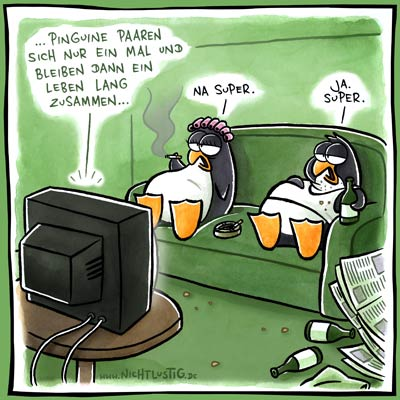
\includegraphics[height=4cm]{./pictures/bild}
			\label{fig:Balkenwaage}}
		\hspace{2cm}
		\subfigure[Federwaage \cite{aaaaaaaaaaa}]
			{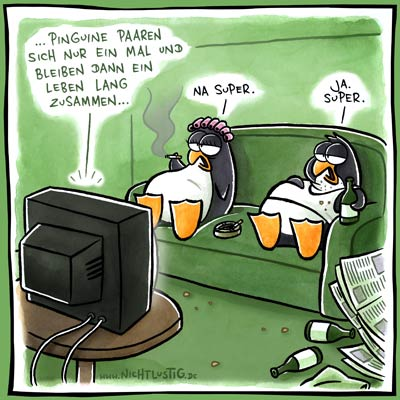
\includegraphics[height=4cm]{./pictures/bild}
			\label{fig:Federwaage}}
		\caption{Balkenwaage und Federwaage}
\end{figure}

Ein \marg{Wügezelle}
sehr weit verbreitetes Wügeprinzip ist die Wügezelle. Hier wird die Verformung eines Federkürpers (i.d.R. aus Metall) mit \ac{DMS} gemessen (siehe Abb. \ref{fig:Federwaage}). \ac{DMS} ündern ihren elektrischen Widerstand, wenn sie verformt werden. Durch geeignete mechanische Konstruktion und Beschaltung kann schliesslich ein zum Gewicht proportionales Signal erzeugt werden. Wügezellen werden in Waagen aller Grüssenordnungen von Haushaltswaagen bis hin zu Kranwaagen eingesetzt.

Für \marg{Doppel-Biegebalken}
kleine Lasten wird der Federkürper einer Wügezelle meist als Doppelbiegebalken ausgeführt. Abb. \ref{fig:Federwaage} zeigt als Beispiel eine solche Wügezelle. Die Doppel\-balken-Konstruktion kann als eine Parallel-Aufhüngung mit vier elastischen Gelenken betrachtet werden. Dadurch kann sich der bewegliche Teil der Wügezelle nur in vertikaler Richtung bewegen und sich nicht neigen. Die Doppelbalken-Wügezelle ist deshalb nur auf Krüfte in vertikaler Richtung empfindlich. Siehe dazu auch \cite{patentYamato}.

\section{asdfsda asdfsd asdfsad}
sadf \marg{sadf s adf asdf }
Lorem ipsum dolor sit amet. Lorem ipsum dolor sit amet, consetetur sadipscing elitr, sed diam nonumy eirmod tempor invidunt ut labore et dolore magna aliquyam erat, sed diam voluptua. At vero eos et accusam  \ref{sec:definitionen}).

\section{asdfsda asdfsd}
sadf \marg{sadf s adf asdf }
Lorem ipsum dolor sit amet. Lorem ipsum dolor sit amet, consetetur sadipscing elitr, sed diam nonumy eirmod tempor invidunt ut labore et dolore magna aliquyam erat, sed diam voluptua. At vero eos et accusam  

Komerziell \marg{sdf sdf asdf}
Lorem ipsum dolor sit amet. Lorem ipsum dolor sit amet, consetetur sadipscing elitr, sed diam nonumy eirmod tempor invidunt ut labore et dolore magna aliquyam erat, sed diam voluptua. At vero eos et accusam  \cite{dynamic}.
 